\section{Extended evaluation of privacy vs overheads}
\label{sec:eval-extended}

\begin{figure}[t]
    \centering
    \begin{subfigure}{0.49\columnwidth}
      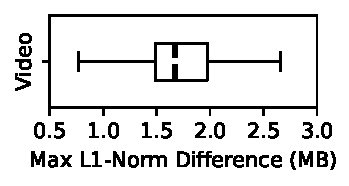
\includegraphics[width=\textwidth]{neighboring_distances_barplot_video.pdf}
%      \caption{Video streaming}
%      \label{subfig:sensitivity-comparison-video}
    \end{subfigure}
    \hfill
    \begin{subfigure}{0.49\columnwidth}
      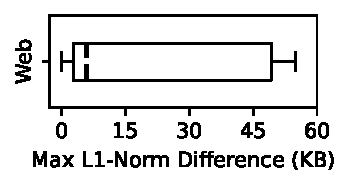
\includegraphics[width=\textwidth]{neighboring_distances_barplot_web.pdf}
%      \caption{Web service}
%      \label{subfig:sensitivity-comparison-web}
    \end{subfigure}
    \caption{\update{Distribution of the difference in buffering queue lengths
    for application stream pairs.}
    }
    \vspace{-0.2cm}
    \label{fig:sensitivity-comparison}
\end{figure}

\begin{figure}[t]
    \centering
    \begin{subfigure}{0.49\columnwidth}
        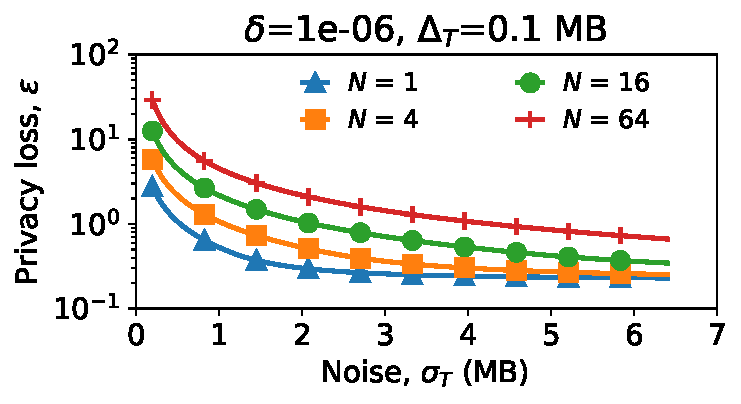
\includegraphics[width=\textwidth]{privacy_loss_VS_noise_std_low_sensitivity_updated.pdf}
        \caption{Noise vs privacy loss}
        \label{subfig:low-sens-epsilon-sigma}
    \end{subfigure}
    \hfill
    \begin{subfigure}{0.49\columnwidth}
        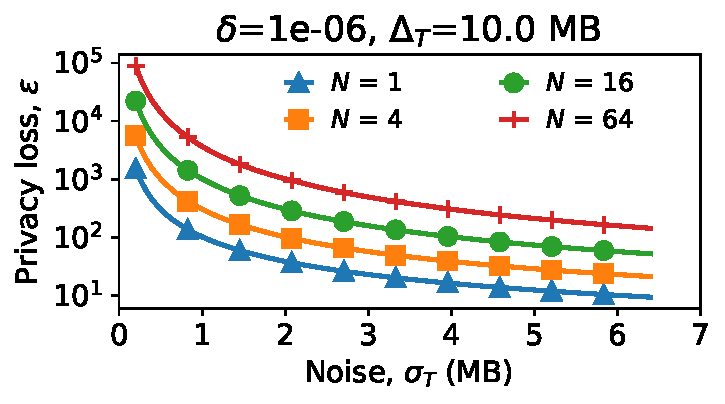
\includegraphics[width=\textwidth]{privacy_loss_VS_noise_std_high_sensitivity_updated.pdf}
        \caption{Noise vs privacy loss}
        \label{subfig:high-sens-epsilon-sigma}
    \end{subfigure}
    \hfill
    %\begin{subfigure}{0.32\textwidth}
    %      \centering
    %
    %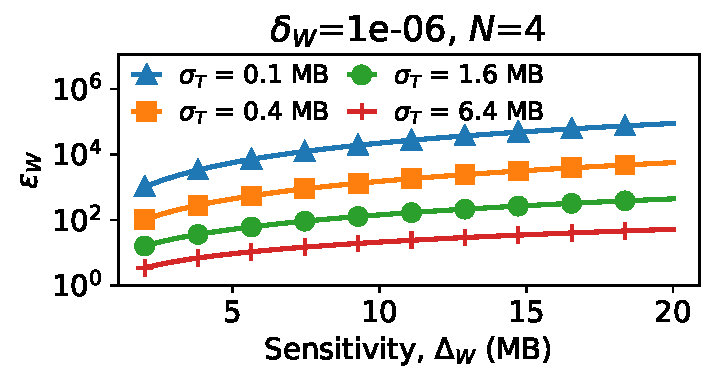
\includegraphics[width=\textwidth]{plots/privacy_loss_VS_sensitivity_high_sensitivity.pdf}
    %      \caption{Sensitivity vs privacy loss}
    %      \label{subfig:high-sens-epsilon-sensitivity}
    %      \end{subfigure}
\begin{subfigure}{0.49\columnwidth}
    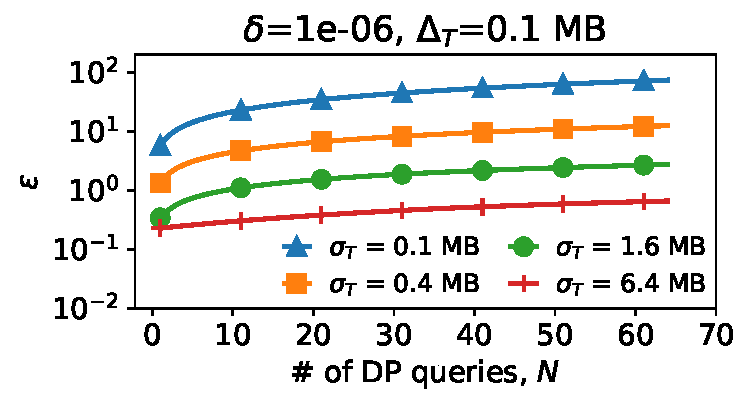
\includegraphics[width=\textwidth]{privacy_loss_VS_query_num_low_sensitivity_updated.pdf}
    \caption{\# DP queries vs privacy loss}
    \label{subfig:low-sens-epsilon-queries}
\end{subfigure}
\hfill
\begin{subfigure}{0.49\columnwidth}
    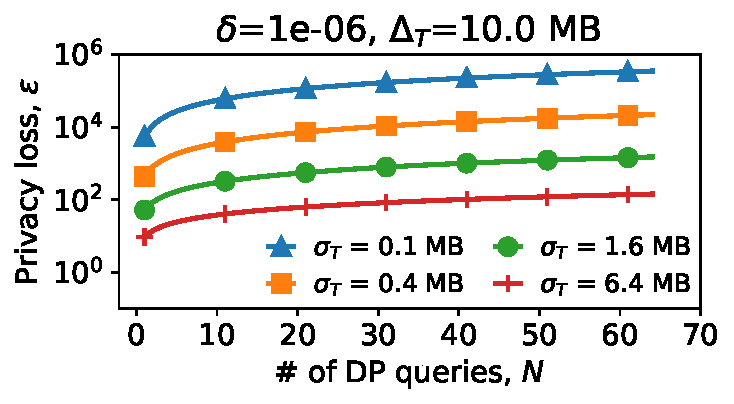
\includegraphics[width=\textwidth]{privacy_loss_VS_query_num_high_sensitivity_updated.pdf}
    \caption{\# DP queries vs privacy loss}
    \label{subfig:high-sens-epsilon-queries}
\end{subfigure}
%    \begin{subfigure}{0.32\textwidth}
    %    \centering
    %
    %
    %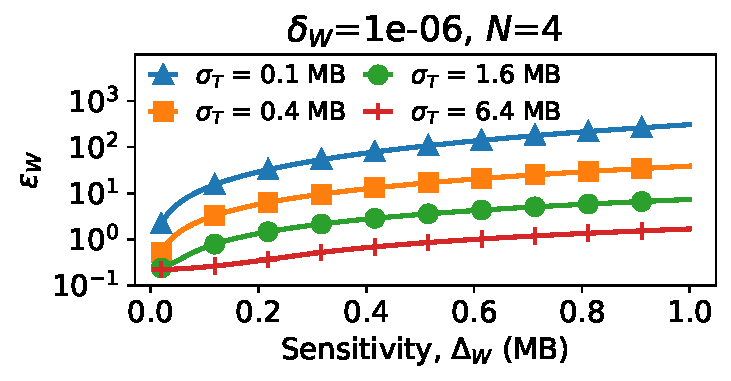
\includegraphics[width=\textwidth]{plots/privacy_loss_VS_sensitivity_low_sensitivity.pdf}
    %    \caption{Sensitivity vs privacy loss}
    %    \label{subfig:low-sens-epsilon-sensitivity}
    %    \end{subfigure}
\caption{
    \update{Privacy loss vs noise and \# queries for different~$\qsens$.}
    %        Relation between per-window loss ($\varepsilon_\winlen$), noise
    %        ($\sigma_\winlen$), sensitivity ($\ssens$), and number of DP
    %        queries ($\varnumupdates$).
}
\vspace{-0.4cm}
\label{fig:privacy-microbenchmarks-extended}
\end{figure}

{\small
%\Cref{subfig:sensitivity-comparison-video,subfig:sensitivity-comparison-web}
\textbf{Distribution of queue length differences.}
\Cref{fig:sensitivity-comparison} shows the distribution of the
buffering queue length differences generated for each pair of an
application's streams. We use $\winlen$ of 5s
for video streams and 1s for web pages.
%The error bars show the min and max differences, the boxes show the first and
%third quartiles.
The dashed lines show the median, which is \update{1.63 MB} and
\update{6 KB} for videos and web pages, respectively.

\textbf{Privacy loss vs overheads for other \update{$\qsens$}.}
\Cref{fig:privacy-microbenchmarks-extended} shows similar results as
\Cref{fig:privacy-microbenchmarks} for \update{$\qsens$} of 0.1 MB and 10 MB.
%of 0.1 MB and 10 MB.
%the relation between $\varepsilon$, $\sigma_\dpintvl$, $\varnumupdates$ for
%$\ssens$ of 0.1 MB and 10 MB.
%at a lower scale of sensitivity ($\ssens$) for two different
%setups: applications with high sensitivity values (e.g. 10 MB) where the queue
%size undergoes significant changes across different streams and applications
%with low sensitivity (e.g. 0.1 MB).
}

